\section*{Appendix}

\section{Algorithm details}
\label{app:alg}
In this section, we summarize the training and testing procedures of RAIL in Algorithm~\ref{alg:train} and~\ref{alg:test}, respectively.

\begin{algorithm}[hbt!]
\caption{RAIL training}\label{alg:train}
\begin{algorithmic}
\Require{$N$ domains $\{D^{\left(1\right)}, ..., D^{\left(N\right)}\}$, pre-trained CLIP model $\{f_I, f_T\}$}
\Ensure{Ridge regression parameter $\lambda$, random projection function $\phi\left(\cdot\right)$, kernel function $\mathcal{K}\left(\cdot, \cdot\right)$}
\State \textbf{Dataset 1 learning}
\For{training batches in $D^{\left(1\right)}$}
\State Extract features $\mathbf{X}_e^{\left(1\right)} = f_I\left(\mathbf{X}^{\left(1\right)}\right)$
\If{\textbf{Primal:}}
\State Initialize the memory matrix $\mathbf{M}_p^{\left(1\right)}$ using Eqn.~\ref{eqn:M_p}
\State Obtain the primal parameter $\mathbf{W}^{\left(1\right)}$ using Eqn.~\ref{primal_regression}
\EndIf
\If{\textbf{Dual:}}
\State Initialize the memory matrix $\mathbf{M}_d^{\left(1\right)}$, label matrix $\mathbf{C}^{\left(1\right)}$ \& kernel $\mathbf{K}^{\left(1\right)}$ by Theorem~\ref{dual_theorem}
\State Obtain the dual parameter $\boldsymbol{\alpha}^{\left(1\right)}$ using Eqn.~\ref{eqn:alpha_update}
\EndIf
\EndFor

\State \textbf{Incremental learning}
\For{$D^{\left(n\right)}$ in $\{D^{\left(2\right)}, ..., D^{\left(N\right)}\}$}
\For{training batches in $D^{\left(1\right)}$}
\State Extract features $\mathbf{X}_e^{\left(n\right)} = f_I\left(\mathbf{X}^{\left(n\right)}\right)$
\If{\textbf{Primal:}}
\State Update the memory matrix $\mathbf{M}_p^{\left(n\right)}$ using Eqn.\ref{M_primal}
\State Update the primal parameter $\mathbf{W}^{\left(n\right)}$ using Eqn.~\ref{w_update}
\EndIf
\If{\textbf{Dual:}}
\State Update the memory matrix $\mathbf{M}_d^{\left(n\right)}$, label matrix $\mathbf{C}^{\left(n\right)}$ \& kernel $\mathbf{K}^{\left(n\right)}$ by Theorem~\ref{dual_theorem}
\State Update the dual parameter $\boldsymbol{\alpha}^{\left(n\right)}$ using Eqn.~\ref{eqn:alpha_update}
\EndIf
\EndFor
\EndFor
\end{algorithmic}
\end{algorithm}

\begin{algorithm}[hbt!]
\caption{RAIL testing}\label{alg:test}
\begin{algorithmic}
\Require{Test dataset $D_{\text{test}}$, CLIP model $\{f_I, f_T\}$, trained RAIL-Adapter $R_{ad}\left(\cdot\right)$, cross-domain label set $C_N$}
\For{$\mathbf{x}_\text{test} \in D_{\text{test}}$}
    \State Obtain the rough prediction $y^*_\text{zs} = {\operatorname{argmax}}\, \hat{\mathbf{y}}_{zs}$ by Eqn.~\ref{zs_prediction}
    \If{$y^*_\text{zs} \in C_L$}
    \State Obtain RAIL-adapter logits $\hat{\mathbf{y}}_{ad} = R_{ad}\left(f_I\left(\mathbf{x}_\text{test}\right)\right)$
    \State Obtain predicted class based on fusion logits $y^* = {\operatorname{argmax}}\, \hat{\mathbf{y}}_{fs}$ by Eqn.~\ref{fs_prediction}
    \Else
    \State Regard $y^*_\text{zs}$ as the final prediction
  \EndIf
 \EndFor
\end{algorithmic}
\end{algorithm}

\newpage
\section{Connection between primal \& dual ridge regression}
\label{app_regression}
In this section, we introduce the connection between primal and dual forms of ridge regression.

Based on the identity $(\mathbf{P}^{-1} + \mathbf{B}^\top \mathbf{R}^{-1} \mathbf{B})^{-1} \mathbf{B}^\top \mathbf{R}^{-1} = \mathbf{P} \mathbf{B}^\top (\mathbf{B}\mathbf{P}\mathbf{B}^\top + \mathbf{R})^{-1}$, the solution of ridge regression is given by:
\begin{equation}
    \mathbf{W} = (\mathbf{\Phi}^\top \mathbf{\Phi} + \lambda \mathbf{I}_d)^{-1} \mathbf{\Phi}^\top \mathbf{Y} = \mathbf{\Phi}^\top (\mathbf{\Phi} \mathbf{\Phi}^\top + \lambda \mathbf{I}_n)^{-1} \mathbf{Y},
\end{equation}
where the former solution is based on the outer-product of data and the latter one is based on the inner-product of data. Parameter $\mathbf{W}$ can thus be rewritten as: $\mathbf{W} = \mathbf{\Phi}^\top \boldsymbol{\alpha}$ with $\boldsymbol{\alpha} = (\mathbf{\Phi} \mathbf{\Phi}^\top + \lambda \mathbf{I}_n)^{-1} \mathbf{Y}$. In this way, the solution $\mathbf{W}$ is interpreted to lie in the span of the sample-cases, even if the dimensionality of the projected features $\mathbf{\Phi}$ is larger than the number of samples.

Utilizing the kernel method, we never actually require access to the explicit features $\mathbf{\Phi}$, which could be of indefinite dimensions. We obtain the prediction with given data $\mathbf{x}$ by projecting it onto the solution $\mathbf{W}$,
\begin{equation}
    \mathbf{\hat{y}} = \phi\left(\mathbf{x}\right)\mathbf{W}  = \phi\left(\mathbf{x}\right) \mathbf{\Phi}^\top (\mathbf{\Phi} \mathbf{\Phi}^\top + \lambda \mathbf{I}_n)^{-1} \mathbf{Y} = \mathcal{K}\left(\mathbf{x}, \mathbf{X}\right) \boldsymbol{\alpha},
\end{equation}

where \( \mathcal{K}\left(\mathbf{x}_i, \mathbf{x}_j\right) = \phi\left(\mathbf{x}_i\right)^\top \phi\left(\mathbf{x}_j\right) \). What we require here is the choice of kernel function $\mathcal{K}\left(\cdot, \cdot\right)$ instead of explicitly defining the projection function.

\section{Proof of Theorems}
\label{app:proof}
In this section, we provide two mathematical proofs for both Theorem~\ref{primal_theorem} and Theorem~\ref{dual_theorem}.

First, we prove the Theorem~\ref{primal_theorem} from the solution of joint training on $n$ datasets with primal ridge regression:

\begin{equation}
\label{joint_solution}
    \mathbf{W}^{\left(n\right)} = 
    \left(\mathbf{\Phi}^{\left(1:n\right) \top} \mathbf{\Phi}^{\left(1:n\right)} + \lambda \mathbf{I}\right)^{-1} \mathbf{\Phi}^{\left(1:n\right) \top} \mathbf{Y}^{\left(1:n\right)}.
\end{equation}

By decoupling the $n$-th data from previous datasets, the $\mathbf{W}^{\left(n\right)}$ can be written as:

\begin{equation}
\label{eqn:decouple}
\begin{aligned}
\mathbf{W}^{\left(n\right)} 
&= \left(
\begin{bmatrix}
    {\mathbf{\Phi}^{\left(1:n-1\right)\top}} & {\mathbf{\Phi}^{\left(n\right)\top}}
\end{bmatrix}
\begin{bmatrix}
    {\left(\mathbf{\Phi}^{\left(1:n-1\right)}\right)} \\
    {\left(\mathbf{\Phi}^{\left(n\right)}\right)}
\end{bmatrix}
 + \lambda \mathbf{I}\right)^{-1}
 \begin{bmatrix}
    {\mathbf{\Phi}^{\left(1:n-1\right)\top}}  & {\mathbf{\Phi}^{\left(n\right)\top}}
\end{bmatrix}
\begin{bmatrix}
    \mathbf{Y}^{\left(1:n-1\right)} & \mathbf{0} \\
    \mathbf{0} & \mathbf{Y}^{\left(n\right)}
\end{bmatrix} \\
            &=
\left({\mathbf{\Phi}^{\left(1:n-1\right)\top}}      
      {\mathbf{\Phi}^{\left(1:n-1\right)}}  
      + \lambda \mathbf{I}
      +{\mathbf{\Phi}^{\left(n\right)\top}}{\mathbf{\Phi}^{\left(n\right)}}\right)^{-1}
\begin{bmatrix}
    {\mathbf{\Phi}^{\left(1:n-1\right)\top}} \mathbf{Y}^{\left(1:n-1\right)} & {\mathbf{\Phi}^{\left(n\right)\top}}
    \mathbf{Y}^{\left(n\right)}\\
\end{bmatrix}.
\end{aligned}
\end{equation}

We introduce the memory matrix as in the following definition:
\begin{equation}
    \label{eqn:M_p}
    \mathbf{M}_p^{\left(n\right)} = 
    \left(\mathbf{\Phi}^{\left(1:n\right) \top} \mathbf{\Phi}^{\left(1:n\right)} + \lambda \mathbf{I}\right)^{-1},
\end{equation}
which is the matrix inversion term of Eqn~\ref{joint_solution}. \\
Noticing that $\mathbf{M}_p^{\left(n-1\right)} = \left({\mathbf{\Phi}^{\left(1:n-1\right)\top}}      
{\mathbf{\Phi}^{\left(1:n-1\right)}}  
+ \lambda \mathbf{I}\right)^{-1}$, 
by Woodbury matrix identity where  $\left(\mathbf{A} + \mathbf{UCV}\right)^{-1} = \mathbf{A}^{-1} - \mathbf{A}^{-1} \mathbf{U} \left(\mathbf{C}^{-1} + \mathbf{V} \mathbf{A}^{-1} \mathbf{U}\right)^{-1} \mathbf{V} \mathbf{A}^{-1}$ and treating $\mathbf{M}_p^{\left(n-1\right)}$ as $\mathbf{A}^{-1}$, the memory at $n$-th step can be further defined as a recursive solution:
\begin{equation}
\label{eqn:memory_p}
\mathbf{M}_p^{\left(n\right)} =
 \mathbf{M}_p^{\left(n-1\right)} - \mathbf{M}_p^{\left(n-1\right)} \mathbf{\Phi}^{\left(n\right)\top} \left(\mathbf{I} + \mathbf{\Phi}^{\left(n\right)} \mathbf{M}_p^{\left(n-1\right)} \mathbf{\Phi}^{\left(n\right)\top}\right)^{-1} \mathbf{\Phi}^{\left(n\right)} \mathbf{M}_p^{\left(n-1\right)}.
\end{equation}

Thus, the parameter $\mathbf{W}^{\left(n\right)}$ is derived as
\begin{equation}
\label{eqn:w_n_derive}
    \mathbf{W}^{\left(n\right)} = 
    \begin{bmatrix}
    \mathbf{M}_p^{\left(n\right)} {\mathbf{\Phi}^{\left(1:n-1\right)\top}} \mathbf{Y}^{\left(1:n-1\right)} &
    \mathbf{M}_p^{\left(n\right)} {\mathbf{\Phi}^{\left(n\right)\top}} \mathbf{Y}^{\left(n\right)}
    \end{bmatrix}.
\end{equation}

% Noticing that $\mathbf{W}^{\left(n-1\right)} = \mathbf{M}_p^{\left(n-1\right)} {\mathbf{\Phi}^{\left(1:n-1\right)\top}} \mathbf{Y}^{\left(1:n-1\right)}$. 
Denotes the left submatrix $\mathbf{M}_p^{(n)} \mathbf{\Phi}^{(1:n-1)\top} \mathbf{Y}^{(1:n-1)}$ as $\mathbf{H}$. By substituting Eqn~\ref{eqn:memory_p} into~\ref{eqn:w_n_derive},
\begin{equation}
    \mathbf{H} = 
    \mathbf{W}^{\left(n-1\right)} - \mathbf{M}_p^{(n-1)} \mathbf{\Phi}^{(n)\top} \left(\mathbf{I} + \mathbf{\Phi}^{(n)} \mathbf{M}_p^{(n-1)} \mathbf{\Phi}^{(n)\top}\right)^{-1}
   \mathbf{\Phi}^{(n)} \mathbf{W}^{\left(n-1\right)}.
\end{equation}
     
Based on the identity of $\left(\mathbf{I} + \mathbf{P}\right)^{-1}=\mathbf{I} - \left(\mathbf{I} + \mathbf{P}\right)^{-1}\mathbf{P}$, it is further derived as:
% \begin{equation}
%     \begin{aligned}
%     \mathbf{H} = 
%     \mathbf{W}^{\left(n-1\right)} - \left(\mathbf{M}_p^{(n-1)} -\mathbf{M}_p^{(n-1)}\mathbf{\Phi}^{(n)\top}\left(\mathbf{I} + \mathbf{\Phi}^{(n)} \mathbf{M}_p^{(n-1)} \mathbf{\Phi}^{(n)\top}\right)^{-1} \mathbf{\Phi}^{(n)} 
%     \mathbf{M}_p^{(n-1)}\right)
%    \mathbf{\Phi}^{(n)\top}\mathbf{\Phi}^{(n)} \mathbf{W}^{\left(n-1\right)}. 
%     \end{aligned}
% \end{equation}

\begin{equation}
    \mathbf{H} = 
    \mathbf{W}^{\left(n-1\right)} - \mathbf{M}_p^{(n)}\mathbf{\Phi}^{(n)\top}
    \mathbf{\Phi}^{(n)}\mathbf{W}^{\left(n-1\right)}. 
\end{equation}

Thus, 
\begin{equation}
    \mathbf{W}^{\left(n\right)} = 
\begin{bmatrix}
    {\mathbf{W}^{\left(n-1\right)}- \mathbf{M}_p^{\left(n\right)} \mathbf{\Phi}^{\left(n\right)\top}\mathbf{\Phi}^{\left(n\right)}\mathbf{W}^{\left(n-1\right)}} & \mathbf{M}_p^{\left(n\right)}\mathbf{\Phi}^{\left(n\right)\top}\mathbf{Y}^{\left(n\right)} \\
\end{bmatrix}.
\end{equation}
The Theorem~\ref{primal_theorem} is proved.

Next, we prove the Theorem~\ref{dual_theorem} as follows. We use the few-shot features $\mathbf{X}_e$ as the class-prototypes as default. The solution of joint training on $n$ datasets with dual form ridge regression is shown as:
\begin{equation}
\label{eqn:dual_joint}
\boldsymbol{\alpha}^{\left(n\right)} = \left(\mathcal{K}\left(\mathbf{X}_e^{\left(1:n\right)}, \mathbf{X}_e^{\left(1:n\right)}\right) + \lambda \mathbf{I}\right)^{-1}\mathbf{Y}^{\left(1:n\right)}.
\end{equation}

Define the memory matrix $\mathbf{M}_d$ as the concatenation of class-prototypes from learned domains, the memory matrix at $n$-th step is obtained by:
\begin{equation}
    \mathbf{M}_d^{\left(n\right)} = 
    \begin{bmatrix} 
    \mathbf{M}_d^{\left(n-1\right)} & \mathbf{X}_e^{\left(n\right)} 
    \end{bmatrix}.
\end{equation}

The kernel matrix at $n$-th step for $\boldsymbol{\alpha}^{\left(n\right)}$ can be partitioned as:
\begin{equation}
\begin{aligned}
    \mathbf{K}^{\left(n\right)} 
        &= \mathcal{K}\left(\mathbf{X}_e^{\left(1:n\right)}, \mathbf{X}_e^{\left(1:n\right)}\right) \\
        &= \begin{bmatrix}
            \mathcal{K}\left(\mathbf{X}_e^{\left(1:n-1\right)}, \mathbf{X}_e^{\left(1:n-1\right)}\right) & \mathcal{K}\left(\mathbf{X}_e^{\left(n\right)}, \mathbf{M}_d^{\left(n-1\right)}\right)^\top  \\
             \mathcal{K}\left(\mathbf{X}_e^{\left(n\right)}, \mathbf{M}_d^{\left(n-1\right)}\right) & \mathcal{K}\left(\mathbf{X}_e^{\left(n\right)}, \mathbf{X}_e^{\left(n\right)}\right)
            \end{bmatrix} \\
        &= \begin{bmatrix}
            \mathbf{K}^{\left(n-1\right)} & \mathcal{K}\left(\mathbf{X}_e^{\left(n\right)}, \mathbf{M}_d^{\left(n-1\right)}\right)^\top  \\
             \mathcal{K}\left(\mathbf{X}_e^{\left(n\right)}, \mathbf{M}_d^{\left(n-1\right)}\right) & \mathcal{K}\left(\mathbf{X}_e^{\left(n\right)}, \mathbf{X}_e^{\left(n\right)}\right)
            \end{bmatrix}.
\end{aligned}
\end{equation}

It indicates that the kernel matrix updates recursively along the diagonal by kernel matrices of the intra-domain covariance within $\mathbf{X}_e^{\left(n\right)}$ and the inter-domain covariance between $\mathbf{X}_e^{\left(n\right)}$ and the memory $\mathbf{M}_d^{\left(n-1\right)}$. The kernel matrix $\mathbf{K}$ therefore memorizes all the covariance information of learned domains. We further denote $\mathbf{Y}^{\left(1:n\right)}$ as $\mathbf{C}^{\left(n\right)}$, which is updated by:
\begin{equation}
    \mathbf{C}^{\left(n\right)} = 
    \begin{bmatrix} 
    \mathbf{C}^{\left(n-1\right)} & \mathbf{0} \\
    \mathbf{0} & \mathbf{Y}^{\left(n\right)}
    \end{bmatrix},
\end{equation}
where the matrix $\mathbf{Y}^{\left(n\right)}$ consists of one-hot labels that are disjoint with those in previous $n-1$ domains. In this way, the parameter $\boldsymbol{\alpha}^{\left(n\right)}$ is solved by updating $\mathbf{K}^{\left(n\right)}$ and $\mathbf{C}^{\left(n\right)}$, resulting in an identical solution to the one of joint learning in Eqn.~\ref{eqn:dual_joint}. Thus, the Theorem~\ref{dual_theorem} is proved.

\section{Implementation details}
\label{app:implementation}
In this section, we introduce the implementation details, including model configuration, hardware setup, and hyperparamter selection. We use the pre-trained CLIP~\cite{radford2021learning} model of the ViT-B/16 image encoder~\cite{dosovitskiy2021an}. All the results are conducted on Ubuntu 20.04 with Intel Core i9-13900K CPU with a single RTX 4090Ti GPU by the average of 3 runs. We conduct a grid search for the regularization parameter $\lambda$ over the range ${10^{-6}, 10^{-5}, ..., 1}$ and the RBF kernel bandwidth over the range ${10^{-6}, 10^{-5}, ..., 10}$. The optimal values are determined by minimizing the regression error on the validation set of the first domain, without access to future domains. These parameters are then fixed for all subsequent learning steps. We use the simplest prompt template \emph{``A photo of a \{\}.''} for generalization across different domains.

\newpage
\section{Ablation studies}
\label{app:abs}
In this section, we conduct two ablation studies to observe the average performance on 10 domains \textit{w.r.t.} the hidden dimension of RHL and the fusion ratio, respectively.
\subsection{RHL dimension}
\label{app:rhl_dim}
We first ablate the hidden dimension of RHL in primal RAIL over the \emph{``Last''} accuracy in Fig.~\ref{fig:rhl_dim}. It is evident that an increase in the RHL dimension correlates with improved adapter's accuracy. Specifically, increasing the dimension from 1k to 10k leads to notable improvements (from 73.6\% to 79.0\%). However, beyond the 10k threshold, the gain in accuracy becomes saturated. The dimensions of 15k and 20k result the same performance of 79.1\%.  Considering the computational cost associated with higher dimensions, we set the RHL dimension to 15k as default in the experiments.
% , which is enough to keep the projected features expressive.

\begin{figure}[t]
    \centering
    \includegraphics[width=0.5\linewidth]{Figures/dim_line.pdf}
    \caption{RHL dimension vs. \emph{``Last''} accuracy (\%) averaged on 10 domains.}
    \label{fig:rhl_dim}
\end{figure}


\subsection{Fusion ratio}
\label{app:fusion_ratio}
\begin{figure}[t]
    \centering
    \includegraphics[width=0.5\linewidth]{Figures/fusion_line.pdf}
    \caption{Fusion ratio vs. \emph{``Average''} and \emph{``Last''} accuracy (\%) averaged on 10 domains.}
    \label{fig:fusion_line}
\end{figure}

Additionally, we conduct an ablation study of fusion ratio $\beta$ in terms of \emph{``Average''} and \emph{``Last''} accuracy. The \emph{``Transfer''} accuracy is not considered here since $\beta$ does not influence it. From Fig.~\ref{fig:fusion_line}, we observe that the best ratio is $0.8$ for both \emph{``Average''} and \emph{``Last''} scores. Note that when $\beta$ equals to $1$, the performance on seen domains fully relies on the RAIL-Adapter. The \emph{``Last''} accuracy with $\beta=0.8$ surpasses the one of pure RAIL-Adapter performance ($\beta=1$) by 1.9\% and 1.3\% in the primal and dual RAIL, respectively. This result verifies our claim that the cooperation with CLIP's generalization ability can preserve the performance on its confident domains (already having good zero-shot performance) and avoid overfitting on limited domain exemplars.

\section{Detailed performance of RAIL with order-I}
\label{sec:details}
\begin{figure}[t]
    \centering
    \begin{subfigure}[b]{0.48\textwidth}
        \centering
        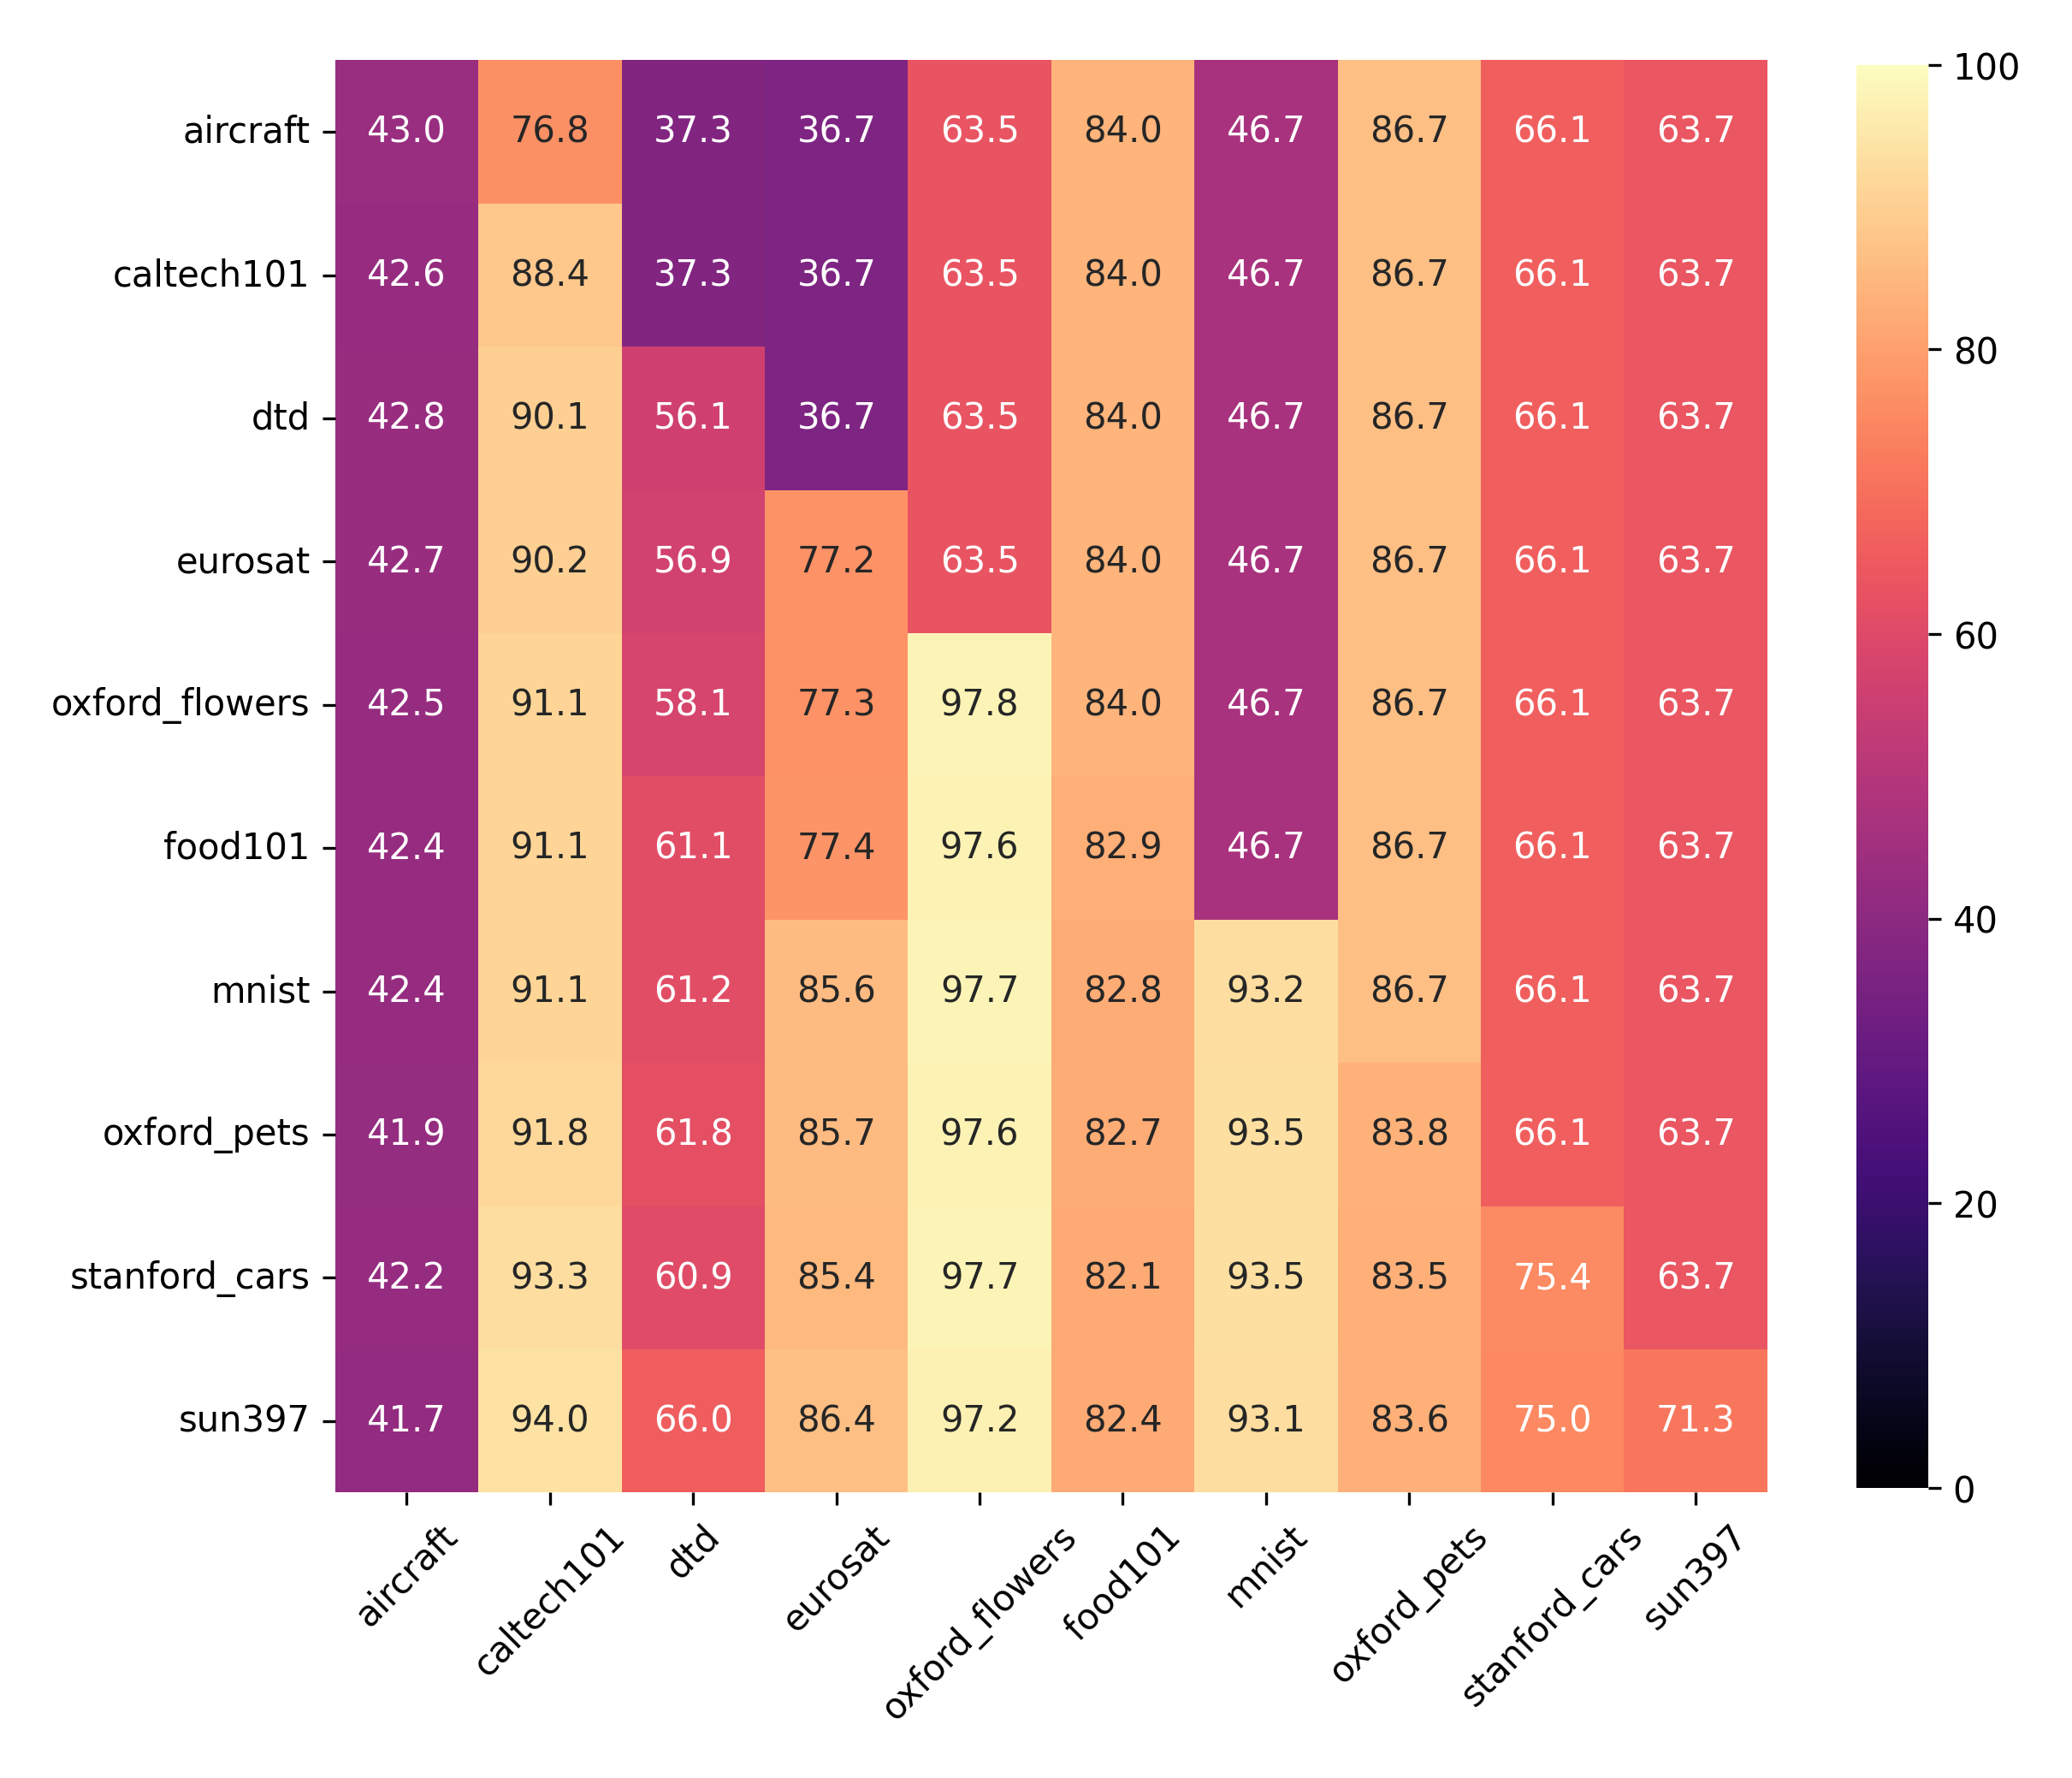
\includegraphics[width=\textwidth]{Figures/Primal_RAIL.png}
        \caption{Primal-RAIL}
    \end{subfigure}
    % \hfill
    \begin{subfigure}[b]{0.48\textwidth}
        \centering
        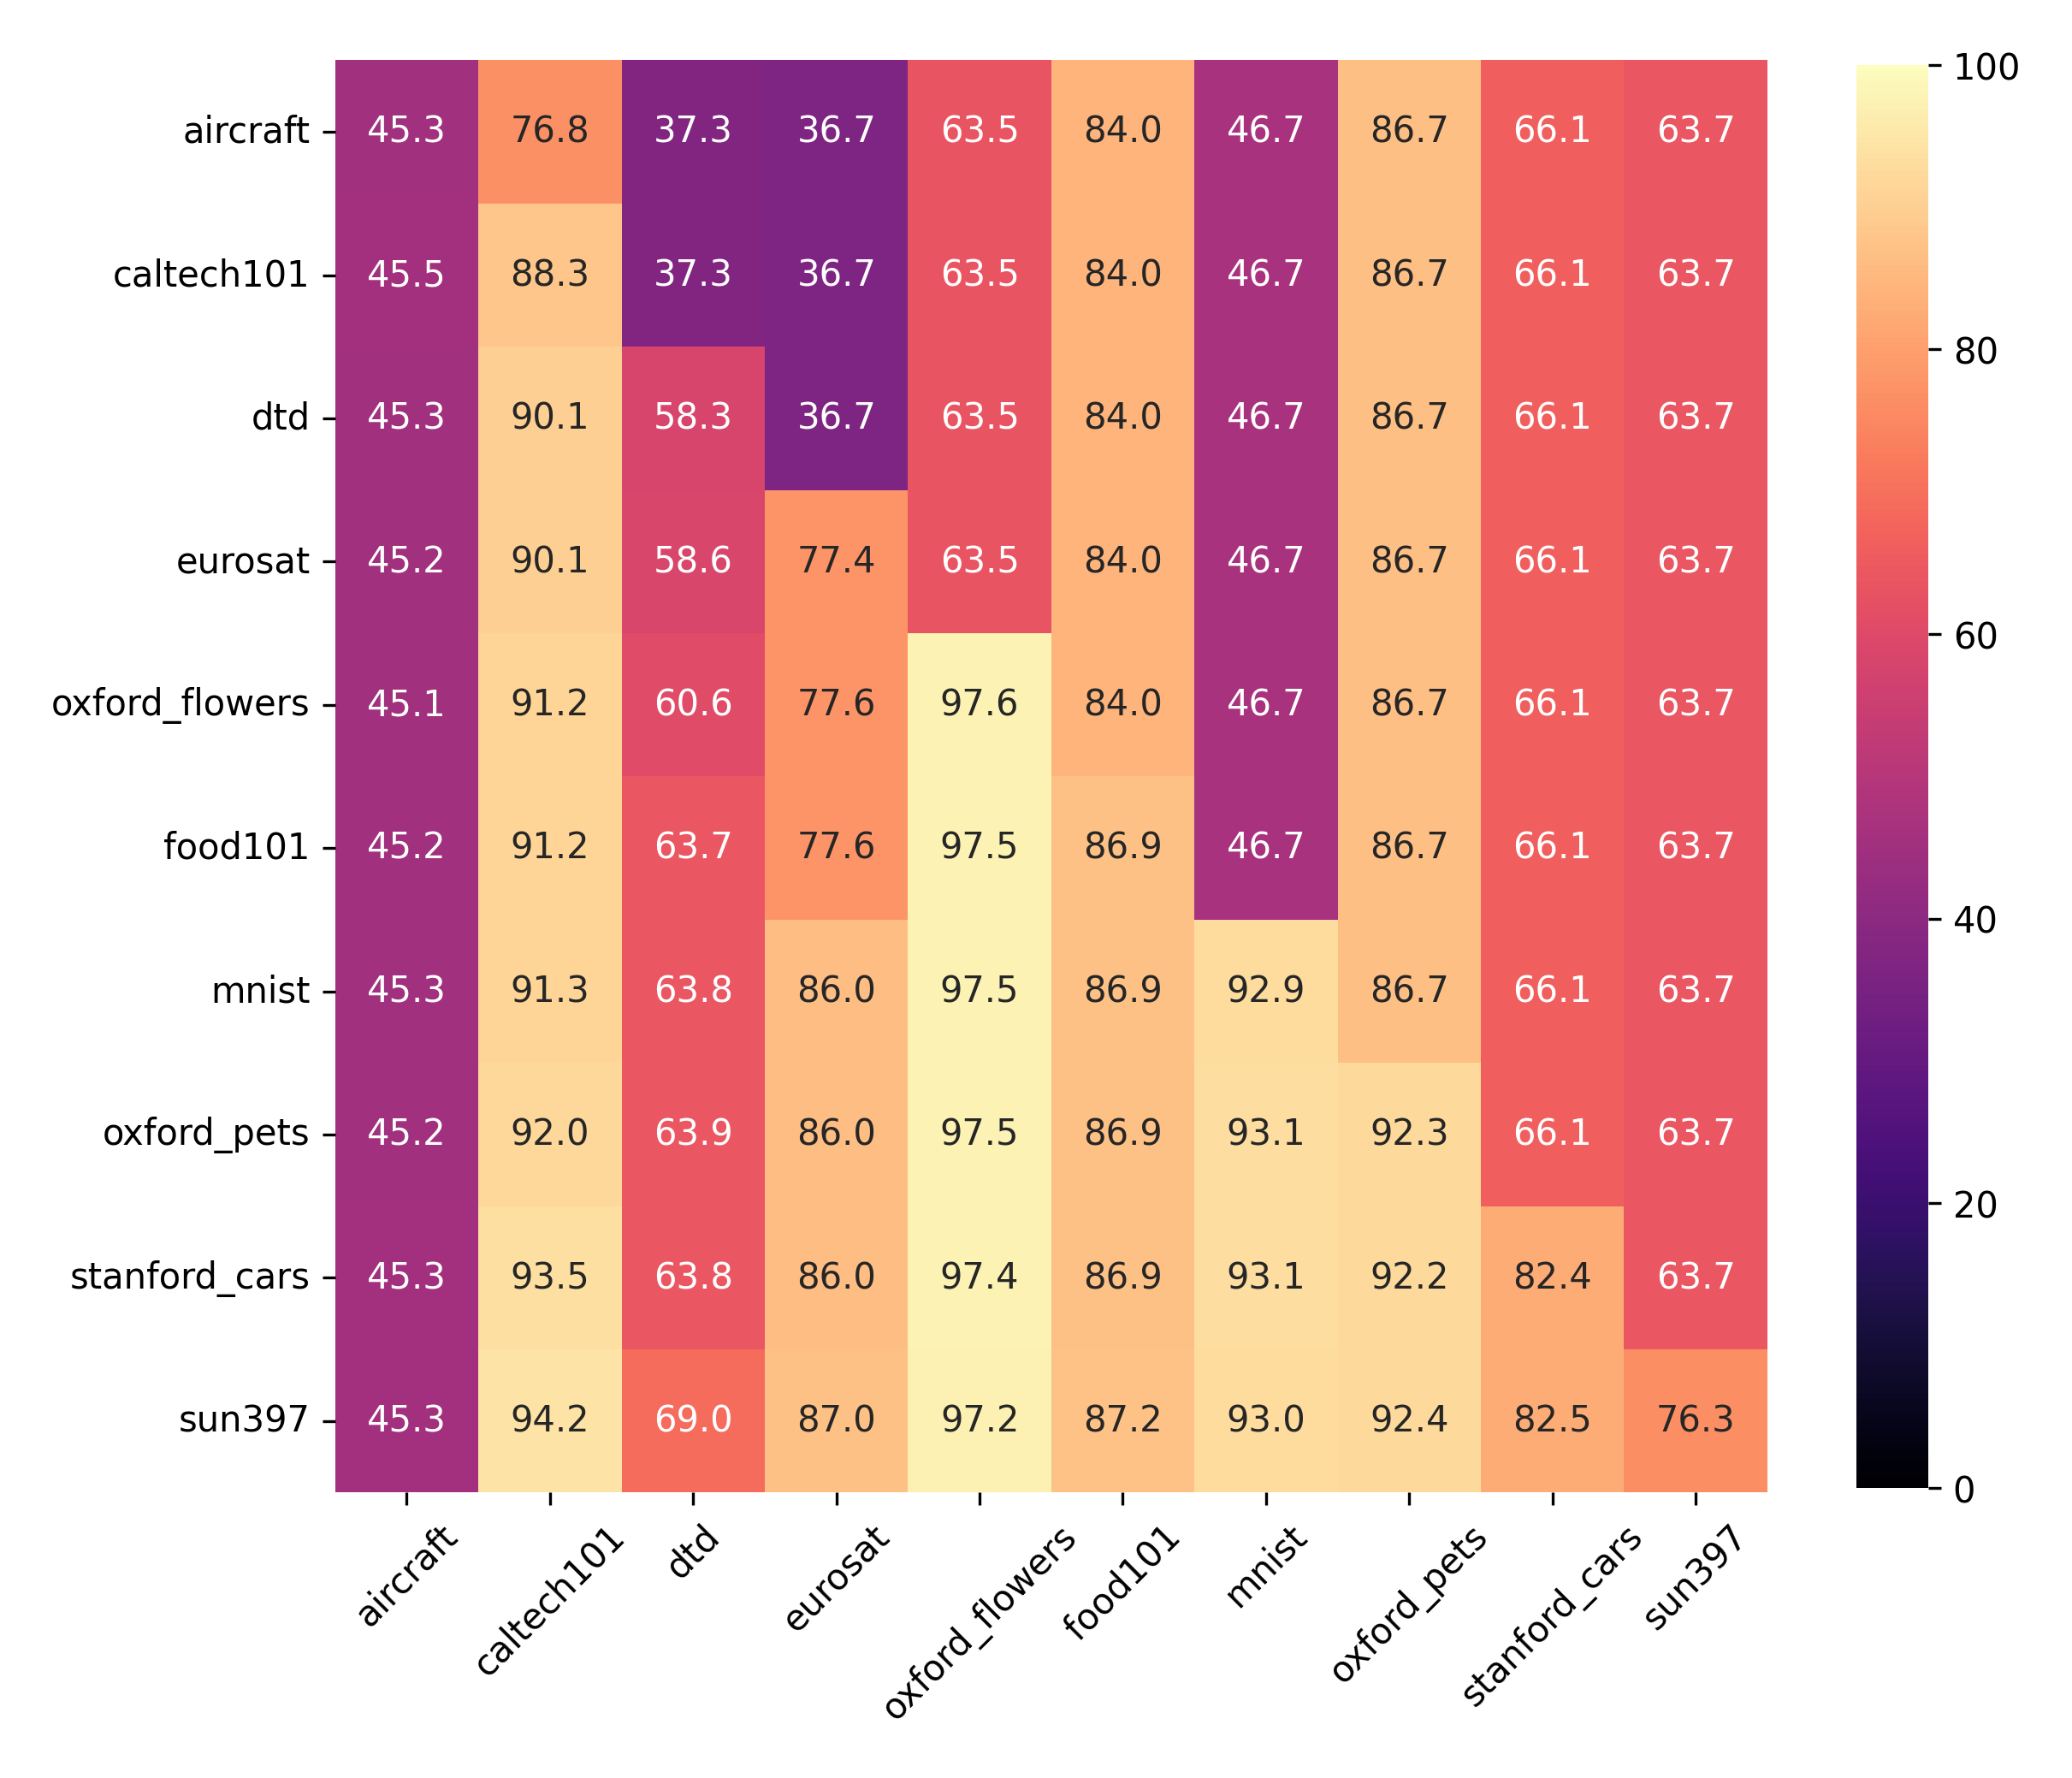
\includegraphics[width=\textwidth]{Figures/Dual_RAIL.png}
        \caption{Dual-RAIL}
    \end{subfigure}
    \caption{Accuracy (\%) of Primal-RAIL and Dual-RAIL in the X-TAIL setting with order-I. Each row denotes the performance on every domain after learning on one domain.}
    \label{fig:detailed_RAIL}
\end{figure}

In this section, we visualize the performance on each domain after every learning step in Fig.~\ref{fig:detailed_RAIL}. The upper-diagonal represents the performance before learning on the corresponding domain, which remains consistent with the zero-shot performance thanks to RAIL's absolute memorization of the zero-shot ability on unseen domains. On the other hand, the performance after learning a specific domain (lower-diagonal) does not degrades. Performance on some domains even improves with the learning step (e.g., Caltech-101), benefiting from our RAIL fusion module design, which reduces OOD errors as more domains are learned, thereby enhancing overall accuracy.

% \section{Comparison of different methods on full-shot MTIL setting}
% \label{app:mtil}
% In this section, we evaluate the performance of RAIL in full-shot MTIL setting, comparing it against the performance of baselines reported in~\cite{yu2024boosting}. In the context of MTIL, where the domain-identity is provided during testing, RAIL is reduced to the structure of multiple domain-specific classifiers trained on each domain separately. The domain-identity guides the test image to the corresponding classifier for within-domain prediction. As shown in~\ref{tab:full_mtil}, RAIL still surpasses all baseline methods in both primal and dual forms. This superior performance can be attributed to the non-linear projection, which significantly enhances the separability of features extracted by CLIP.

% \begin{table}
%     \centering
%     \footnotesize
%     \caption{Comparison with state-of-the-art methods on full-shot MTIL setting in terms of "Transfer", "Average", and "Last" scores (\%). The best results are highlighted with \textbf{bold} style.}
%     \label{tab:full_mtil}
%     \begin{tabular}{b{8em}b{1.6em}b{1.6em}b{1.6em}b{1.6em}b{1.6em}b{1.6em}b{1.6em}b{1.6em}b{1.6em}b{1.6em}b{1.6em}>{\centering\arraybackslash}m{3em}}
%     \toprule
%         \textbf{Method} &  \rot{Aircraft} &  \rot{Caltech101} & \rot{CIFAR100} &\rot{DTD} & \rot{EuroSAT} & \rot{Flower} & \rot{Food101} & \rot{MNIST} & \rot{Pets} & \rot{Cars} & \rot{Sun397} & \textbf{Average}\\
%     \midrule
%           \quad Zero-shot & 24.3 & 88.4 & 68.2 & 44.6 & 54.9 & 71.0 & 88.5 & 59.6 & 89.0 & 64.7 & 65.2 & {\cellcolor{lightgrey}}65.3\\
%           \quad Fine-tune & 62.0 & 95.1 & 89.6 & 79.5 & 98.9 & 97.5 & 92.7 & 99.6 & 94.7 & 89.6 & 81.8 & {\cellcolor{lightgrey}}89.2\\
%     \midrule
%         \multicolumn{11}{l}{\textbf{Transfer}}\\
%           \quad LwF & -- & 74.5 & 56.9 & 39.1 & 51.1 & 52.6 & 72.8 & 60.6 & 75.1 & 30.3 & 55.9 & {\cellcolor{lightgrey}} 58.9\\
%           \quad LwF-VR & -- & 77.1 & 61.0 & 40.5 & 45.3 & 54.4 & 74.6 & 47.9 & 76.7 & 36.3 & 58.6 & {\cellcolor{lightgrey}}57.2\\
%           \quad WiSE-FT & -- & 73.5 & 55.6 & 35.6 & 41.5 & 47.0 & 68.3 & 53.9 & 69.3 & 26.8 & 51.9 & {\cellcolor{lightgrey}}52.3\\
%           \quad ZSCL & -- & 86.0 & 67.4 & \textbf{45.4} & 50.4 & 69.1 & 87.6 & \textbf{61.8} & 86.8 & 60.1 & \textbf{66.8} & {\cellcolor{lightgrey}}68.1\\
%           \quad MoE-Adapter & -- & 87.9 & \textbf{68.2}& 44.4 & 49.9 & 70.7 & \textbf{88.7} & 59.7 & \textbf{89.1} & 64.5 & 65.5 & {\cellcolor{lightgrey}}68.9\\
%           \quad Primal-RAIL & -- & \textbf{88.4}&\textbf{68.2}& 44.6 &\textbf{54.9}&\textbf{71.0}& 88.5 & 59.6 & 89.0 &\textbf{64.7}&65.2& {\cellcolor{lightgrey}}\textbf{69.4}\\
%           % {\cellcolor{lightgrey}}\textbf{69.4(+0.5)}\\
%           \quad Dual-RAIL & -- & \textbf{88.4}&\textbf{68.2}& 44.6 &\textbf{54.9}&\textbf{71.0}& 88.5 & 59.6 & 89.0 &\textbf{64.7}&65.2& {\cellcolor{lightgrey}}\textbf{69.4}\\
%           % {\cellcolor{lightgrey}}\textbf{69.4(+0.5)}\\
          
%     \midrule
%         \multicolumn{11}{l}{\textbf{Average}}\\
%           \quad LwF& 36.3 & 86.9 & 72.0 & 59.0 & 73.7 & 60.0 & 73.6 & 74.8 & 80.0 & 37.3 & 58.1 & {\cellcolor{lightgrey}}64.7\\
%           \quad LwF-VR& 29.6 & 87.7 & 74.4 & 59.5 & 72.4 & 63.6 & 77.0 & 66.7 & 81.2 & 43.7 & 60.7 & {\cellcolor{lightgrey}}65.1\\
%           \quad WiSE-FT& 26.7 & 86.5 & 64.3 & 57.1 & 65.7 & 58.7 & 71.1 & 70.5 & 75.8 & 36.9 & 54.6 & {\cellcolor{lightgrey}}60.7\\
%           \quad ZSCL& 45.1 & 92.0 & 80.1 & 64.3 & 79.5 & 81.6 & \textbf{89.6} & \textbf{75.2} & 88.9 & 64.7 & \textbf{68.0} & {\cellcolor{lightgrey}}75.4\\
%           \quad MoE-Adapter & 50.2 & 91.9 & \textbf{83.1} & 69.4 & 78.9 & 84.0 & 89.1 & 73.7 & 89.3 & 67.7 & 66.9 & {\cellcolor{lightgrey}} 76.7\\
%           \quad Primal-RAIL & 51.9 & 95.8 & 80.1 & 70.3 & 81.1 & 86.1 & 89.0 & 73.9 & \textbf{90.2} & 68.4 & 66.4 & {\cellcolor{lightgrey}}77.6\\
%           % {\cellcolor{lightgrey}}71.9(+0.5)\\
%           \quad Dual-RAIL & \textbf{52.5} & \textbf{96.0} & 80.6 & \textbf{70.4} & \textbf{81.3} & \textbf{86.3} & 89.1 & 73.9 & \textbf{90.2} & \textbf{68.5} & 66.5 & {\cellcolor{lightgrey}}\textbf{77.8}
%           % {\cellcolor{lightgrey}}\textbf{72.3(+0.9)}
%  \\
%     \midrule
%         \multicolumn{11}{l}{\textbf{Last}}\\
%           \quad LwF& 26.3 & 87.5 & 71.9 & 66.6 & 79.9 & 66.9 & 83.8 & \textbf{99.6} & 92.1 & 66.1 & 80.4 & {\cellcolor{lightgrey}}74.6\\
%           \quad LwF-VR& 20.5 & 89.8 & 72.3 & 67.6 & 85.5 & 73.8 & 85.7 & \textbf{99.6} & 93.1 & 73.3 & 80.9 & {\cellcolor{lightgrey}}76.6\\
%           \quad WiSE-FT& 27.2 & 90.8 & 68.0 & 68.9 & 86.9 & 74.0 & 87.6 & \textbf{99.6} & 92.6 & 77.8 & \textbf{81.3} & {\cellcolor{lightgrey}}77.7\\
%           \quad ZSCL& 40.6 & 92.2 & 81.3 & 70.5 & 94.8 & 90.5 & \textbf{91.9} & 98.7 & \textbf{93.9} & 85.3 & 80.2 & {\cellcolor{lightgrey}}83.6\\
%           \quad MoE-Adapter & 49.8 & 92.2 & \textbf{86.1} & 78.1 & 95.7 & 94.3 & 89.5 & 98.1 & 89.9 & 81.6 & 80.0 & {\cellcolor{lightgrey}}85.0\\
%           \quad Primal-RAIL & 51.9 & 96.5 & 82.8 & 80.0 & 96.0 & 98.7 & 89.7 & 98.8 & 93.3 & 84.8 & 78.7 & {\cellcolor{lightgrey}}86.5\\
%           % {\cellcolor{lightgrey}}77.2(+1.1)\\
%           \quad Dual-RAIL & \textbf{52.5} & \textbf{96.8} & 83.3 & \textbf{80.1} & \textbf{96.4} & \textbf{99.0} & 89.9 & 98.8 & 93.5 & \textbf{85.5} & 79.2 & {\cellcolor{lightgrey}}\textbf{86.8} \\
%           % {\cellcolor{lightgrey}}\textbf{77.9(+1.8)} \\
%     \bottomrule
%     \end{tabular}
% \end{table}

% \begin{table}[h]
%     \centering
%     \caption{Accuracy(\%) of the LwF method on X-TAIL with order-I.}
%     \label{tab:lwf_fs_merged}
%     \begin{tabular}{b{5em}b{2em}b{2em}b{2em}b{2em}b{2em}b{2em}b{2em}b{2em}b{2em}b{2em}b{2em}}
%     \toprule
%         &  \rot{Aircraft} &  \rot{Caltech101} & \rot{DTD} & \rot{EuroSAT} & \rot{Flower} & \rot{Food101} & \rot{MNIST} & \rot{Pets} & \rot{Cars} & \rot{Sun397} & \\
%         \midrule
% \textbf{Transfer} & nan & 66.6 & 26.9 & 19.5 & 51.0 & 78.4 & 26.6 & 68.9 & 35.5 & 56.1 & \cellcolor{blue!25}\textbf{47.7}\\
% \midrule
% Aircraft & 35.1 & 66.6 & 26.6 & 23.8 & 47.5 & 78.0 & 25.7 & 70.8 & 32.6 & 59.2\\
% Caltech101 & 26.1 & 85.3 & 27.1 & 21.3 & 55.0 & 80.4 & 27.2 & 72.0 & 38.6 & 62.1\\
% DTD & 25.1 & 83.9 & 49.3 & 13.3 & 53.6 & 79.2 & 28.2 & 76.9 & 39.3 & 57.6\\
% EuroSAT & 29.3 & 77.8 & 46.6 & 44.9 & 48.0 & 78.0 & 30.4 & 77.3 & 37.7 & 50.7\\
% Flowers & 27.4 & 79.6 & 45.4 & 50.3 & 91.9 & 76.5 & 22.6 & 71.5 & 33.2 & 52.8\\
% Food & 20.3 & 84.6 & 34.3 & 51.7 & 58.3 & 83.8 & 25.4 & 52.4 & 33.1 & 55.9\\
% MNIST & 17.6 & 84.3 & 39.7 & 47.2 & 69.7 & 82.7 & 40.9 & 61.4 & 35.5 & 56.7\\
% OxfordPet & 20.2 & 80.5 & 35.1 & 32.4 & 73.5 & 81.5 & 31.5 & 73.0 & 34.2 & 53.3\\
% StanfordCars & 20.6 & 82.2 & 39.6 & 29.2 & 76.1 & 82.3 & 51.1 & 75.4 & 78.7 & 56.9\\
% SUN397 & 20.9 & 83.1 & 47.5 & 38.2 & 75.5 & 84.7 & 50.1 & 78.0 & 75.8 & 74.6 & \cellcolor{orange!25}\textbf{62.8}\\
% \midrule
% \textbf{Average} & 24.3 & 80.8 & 39.1 & 35.2 & 64.9 & 80.7 & 33.3 & 70.9 & 43.9 & 58.0 & \cellcolor{red!25}\textbf{53.1}\\
%     \bottomrule
%     \end{tabular}
% \end{table}

% \begin{table}[h]
%     \centering
%     \caption{Accuracy(\%) of the WiSE-FT method on X-TAIL with order-I.}
%     \label{tab:lwf_fs_merged}
%     \begin{tabular}{b{5em}b{2em}b{2em}b{2em}b{2em}b{2em}b{2em}b{2em}b{2em}b{2em}b{2em}b{2em}}
%     \toprule
%         &  \rot{Aircraft} &  \rot{Caltech101} & \rot{DTD} & \rot{EuroSAT} & \rot{Flower} & \rot{Food101} & \rot{MNIST} & \rot{Pets} & \rot{Cars} & \rot{Sun397} & \\
%         \midrule
% \textbf{Transfer} & -- & 70.1 & 31.9 & 25.3 & 56.3 & 79.8 & 29.9 & 74.9 & 45.6 & 56.8 & \cellcolor{blue!25}\textbf{52.3}\\
% \midrule
% Aircraft & 31.9 & 70.1 & 33.2 & 31.9 & 60.1 & 84.1 & 30.9 & 82.6 & 51.1 & 63.5\\
% Caltech101 & 30.2 & 81.3 & 30.5 & 24.1 & 56.8 & 81.4 & 29.0 & 76.8 & 50.1 & 61.2\\
% DTD & 28.7 & 79.2 & 50.1 & 20.0 & 54.3 & 78.2 & 29.7 & 77.1 & 48.4 & 55.8\\
% EuroSAT & 30.8 & 77.6 & 48.6 & 38.7 & 53.9 & 79.3 & 31.6 & 77.2 & 47.8 & 52.8\\
% Flowers & 26.7 & 77.9 & 43.3 & 46.3 & 88.4 & 76.1 & 29.5 & 70.1 & 40.3 & 52.3\\
% Food & 27.4 & 77.5 & 41.9 & 41.0 & 72.5 & 84.0 & 28.9 & 67.7 & 44.3 & 59.5\\
% MNIST & 26.7 & 76.4 & 42.7 & 37.6 & 74.3 & 83.5 & 40.2 & 73.2 & 43.9 & 57.8\\
% OxfordPet & 24.3 & 74.0 & 37.3 & 29.3 & 74.8 & 81.9 & 32.9 & 72.6 & 38.9 & 53.1\\
% StanfordCars & 23.1 & 74.4 & 38.6 & 23.4 & 74.1 & 82.3 & 30.2 & 72.8 & 76.2 & 55.4\\
% SUN397 & 21.8 & 76.8 & 42.9 & 20.8 & 77.5 & 84.9 & 30.7 & 76.6 & 75.8 & 72.5 & \cellcolor{orange!25}\textbf{58.0}\\
% \midrule
% \textbf{Average} & 27.1 & 76.5 & 40.9 & 31.3 & 68.7 & 81.6 & 31.4 & 74.7 & 51.7 & 58.4 & \cellcolor{red!25}\textbf{54.2}\\
%     \bottomrule
%     \end{tabular}
% \end{table}

% \begin{table}[h]
%     \centering
%     \caption{Accuracy(\%) of the iCaRL method on X-TAIL with order-I.}
%     \label{tab:lwf_fs_merged}
%     \begin{tabular}{b{5em}b{2em}b{2em}b{2em}b{2em}b{2em}b{2em}b{2em}b{2em}b{2em}b{2em}b{2em}}
%     \toprule
%         &  \rot{Aircraft} &  \rot{Caltech101} & \rot{DTD} & \rot{EuroSAT} & \rot{Flower} & \rot{Food101} & \rot{MNIST} & \rot{Pets} & \rot{Cars} & \rot{Sun397} & \\
%         \midrule
% \textbf{Transfer} & nan & 71.7 & 35.0 & 43.0 & 64.4 & 86.9 & 43.9 & 87.8 & 63.7 & 60.0 & \cellcolor{blue!25}\textbf{61.8}\\
% \midrule
% Aircraft & 25.3 & 71.7 & 34.7 & 43.5 & 63.6 & 86.7 & 42.7 & 87.1 & 63.7 & 58.6\\
% Caltech101 & 25.4 & 72.1 & 35.3 & 42.6 & 64.4 & 86.9 & 43.4 & 87.6 & 63.8 & 59.4\\
% DTD & 25.4 & 72.2 & 37.6 & 42.8 & 64.8 & 87.0 & 43.5 & 87.9 & 63.8 & 59.8\\
% EuroSAT & 25.5 & 72.3 & 37.8 & 55.2 & 64.8 & 87.0 & 44.6 & 87.9 & 63.7 & 60.1\\
% Flowers & 25.4 & 72.1 & 37.7 & 55.2 & 65.7 & 87.0 & 44.4 & 88.0 & 63.7 & 60.0\\
% Food & 25.4 & 72.0 & 37.6 & 55.1 & 65.8 & 87.0 & 44.5 & 88.0 & 63.7 & 60.1\\
% MNIST & 25.6 & 72.4 & 38.2 & 55.4 & 65.5 & 87.2 & 81.9 & 88.1 & 63.6 & 60.8\\
% OxfordPet & 25.5 & 72.2 & 38.5 & 55.5 & 65.5 & 87.2 & 81.9 & 88.7 & 63.6 & 60.5\\
% StanfordCars & 25.2 & 71.9 & 38.7 & 55.3 & 65.5 & 87.3 & 81.8 & 88.6 & 63.6 & 60.3\\
% SUN397 & 25.5 & 72.1 & 38.9 & 55.4 & 65.5 & 87.3 & 81.9 & 88.6 & 63.6 & 61.5 & \cellcolor{orange!25}\textbf{64.0}\\
% \midrule
% \textbf{Average} & 25.4 & 72.1 & 37.5 & 51.6 & 65.1 & 87.1 & 59.1 & 88.0 & 63.7 & 60.1 & \cellcolor{red!25}\textbf{61.0}\\
%     \bottomrule
%     \end{tabular}
% \end{table}

% \begin{table}[h]
%     \centering
%     \caption{Accuracy(\%) of the ZSCL method on X-TAIL with order-I.}
%     \label{tab:lwf_fs_merged}
%     \begin{tabular}{b{5em}b{2em}b{2em}b{2em}b{2em}b{2em}b{2em}b{2em}b{2em}b{2em}b{2em}b{2em}}
%     \toprule
%         &  \rot{Aircraft} &  \rot{Caltech101} & \rot{DTD} & \rot{EuroSAT} & \rot{Flower} & \rot{Food101} & \rot{MNIST} & \rot{Pets} & \rot{Cars} & \rot{Sun397} & \\
%         \midrule
% \textbf{Transfer} & -- & 73.3 & 32.6 & 36.8 & 62.1 & 83.8 & 42.1 & 83.6 & 56.5 & 60.2 & \cellcolor{blue!25}\textbf{59.0}\\
% \midrule
% Aircraft & 42.7 & 73.3 & 34.9 & 42.3 & 65.5 & 86.7 & 43.9 & 86.5 & 61.7 & 62.7\\
% Caltech101 & 40.7 & 77.0 & 30.2 & 34.7 & 62.5 & 84.3 & 38.9 & 82.0 & 58.8 & 61.6\\
% DTD & 40.2 & 75.5 & 48.1 & 33.3 & 60.4 & 83.0 & 41.1 & 83.9 & 57.8 & 60.3\\
% EuroSAT & 39.3 & 73.2 & 48.4 & 50.6 & 59.8 & 82.7 & 42.2 & 84.0 & 56.9 & 58.1\\
% Flowers & 36.2 & 73.5 & 42.2 & 43.7 & 85.6 & 82.3 & 41.5 & 80.0 & 52.7 & 56.2\\
% Food & 34.3 & 77.1 & 42.7 & 47.6 & 77.1 & 87.4 & 44.7 & 84.2 & 56.1 & 62.7\\
% MNIST & 34.4 & 76.1 & 43.5 & 45.3 & 77.8 & 87.3 & 56.8 & 84.7 & 55.8 & 61.9\\
% OxfordPet & 29.7 & 74.9 & 37.4 & 36.0 & 74.7 & 86.0 & 51.9 & 82.2 & 52.3 & 58.7\\
% StanfordCars & 29.9 & 74.0 & 36.4 & 36.2 & 72.0 & 86.1 & 51.7 & 81.4 & 77.9 & 59.4\\
% SUN397 & 33.1 & 75.3 & 43.5 & 35.2 & 74.6 & 87.4 & 50.4 & 84.2 & 77.3 & 73.4 & \cellcolor{orange!25}\textbf{63.4}\\
% \midrule
% \textbf{Average} & 36.0 & 75.0 & 40.7 & 40.5 & 71.0 & 85.3 & 46.3 & 83.3 & 60.7 & 61.5 & \cellcolor{red!25}\textbf{60.0}\\
%     \bottomrule
%     \end{tabular}
% \end{table}

% \begin{table}[h]
%     \centering
%     \caption{Accuracy(\%) of the MoE-Adapter method on X-TAIL with order-I.}
%     \label{tab:lwf_fs_merged}
%     \begin{tabular}{b{5em}b{2em}b{2em}b{2em}b{2em}b{2em}b{2em}b{2em}b{2em}b{2em}b{2em}b{2em}}
%     \toprule
%         &  \rot{Aircraft} &  \rot{Caltech101} & \rot{DTD} & \rot{EuroSAT} & \rot{Flower} & \rot{Food101} & \rot{MNIST} & \rot{Pets} & \rot{Cars} & \rot{Sun397} & \\
%         \midrule
% \textbf{Transfer} & -- & 71.0 & 34.9 & 19.2 & 63.0 & 86.6 & 20.0 & 87.2 & 63.7 & 58.6 & \cellcolor{blue!25}\textbf{56.0}\\
% \midrule
% Aircraft & 43.3 & 71.0 & 35.5 & 19.2 & 64.0 & 86.6 & 12.6 & 87.2 & 63.7 & 58.3\\
% Caltech101 & 43.7 & 79.7 & 34.3 & 19.2 & 62.5 & 86.6 & 16.0 & 87.2 & 63.7 & 58.6\\
% DTD & 43.5 & 78.7 & 58.6 & 19.2 & 62.7 & 86.6 & 22.7 & 87.2 & 63.7 & 58.8\\
% EuroSAT & 43.3 & 78.3 & 56.4 & 48.5 & 62.9 & 86.6 & 22.1 & 87.2 & 63.7 & 58.8\\
% Flowers & 43.8 & 78.3 & 58.2 & 47.1 & 92.2 & 86.6 & 23.1 & 87.2 & 63.7 & 58.6\\
% Food & 43.7 & 78.4 & 55.4 & 41.9 & 88.9 & 86.2 & 23.3 & 87.2 & 63.7 & 58.6\\
% MNIST & 44.0 & 78.5 & 54.0 & 43.1 & 87.6 & 86.1 & 82.1 & 87.2 & 63.7 & 58.6\\
% OxfordPet & 43.7 & 78.4 & 54.8 & 40.1 & 80.7 & 85.8 & 82.0 & 87.9 & 63.7 & 58.5\\
% StanfordCars & 43.2 & 78.6 & 55.8 & 36.0 & 78.3 & 86.0 & 81.7 & 87.9 & 78.1 & 58.5\\
% SUN397 & 43.2 & 78.7 & 57.6 & 32.8 & 79.4 & 86.0 & 86.7 & 87.8 & 78.2 & 74.2 & \cellcolor{orange!25}\textbf{70.5}\\
% \midrule
% \textbf{Average} & 43.6 & 77.9 & 52.1 & 34.7 & 75.9 & 86.3 & 45.2 & 87.4 & 66.6 & 60.2 & \cellcolor{red!25}\textbf{63.0}\\
%     \bottomrule
%     \end{tabular}
% \end{table}

% \clearpage
% \begin{table}
%     \centering
%     \caption{Comparison of different CL methods on X-TAIL setting with order II.}
%     \label{tab:main_table_order2}
%     \begin{tabular}{b{6em}b{3em}b{3em}b{3em}}
%     \toprule
%         Method & Transfer & Average & Last\\
%     \midrule
%         LwF & 46.9 & 52.0 & 55.4\\
%         WiSE-FT & 51.1 & 56.9 & 61.5\\
%         iCaRL &  &  & \\
%         ZSCL & 56.9 & 63.6 & 69.4\\ 
%         MoE-Adapter & & & \\
%         Ours (Primal) & & & \\
%         Ours (Dual) & & & \\
%     \bottomrule
%     \end{tabular}
% \end{table}

\section{Comparison of different methods on X-TAIL with order II.}
\label{app:order2}
In this section, we compare different methods in X-TAIL setting with a random order: StanfordCars, Aircraft, OxfordPet, Food, SUN397, MNIST, Flowers, DTD, Caltech101, EuroSAT. As shown in Tab.~\ref{tab:detailed_comparison_order2}, our method again outperforms previous methods on all metrics, reinforcing the conclusions presented in Sec.~\ref{sec:comparison}.

\begin{table}
    \centering
    \footnotesize
    \caption{Comparison of different CL methods on X-TAIL for each domain with order II in terms of "Transfer", "Average", and "Last" scores (\%). The best results are highlighted with \textbf{bold} style.}
    \label{tab:detailed_comparison_order2}
    \begin{tabular}{b{8em}b{1.6em}b{1.6em}b{1.6em}b{1.6em}b{1.6em}b{1.6em}b{1.6em}b{1.6em}b{1.6em}b{1.6em}>{\centering\arraybackslash}m{3em}}
    \toprule
        \textbf{Method} &  \rot{Cars} &  \rot{Aircraft} & \rot{Pets} & \rot{Food} & \rot{SUN397} & \rot{MNIST} & \rot{Flower} & \rot{DTD} & \rot{Caltech101} & \rot{EuroSAT} & \textbf{Average} \\
    \midrule
          \quad Zero-shot & 66.1 & 23.5 & 86.7 & 84.0 & 63.7 & 46.7 & 63.6 & 37.3 & 76.8 & 36.7 & {\cellcolor{lightgrey}}58.5 \\
          \quad Fine-tune & 77.4 & 39.6 & 84.4 & 85.5 & 72.4 & 95.1 & 95.4 & 68.2 & 93.3 & 89.2 & {\cellcolor{lightgrey}}80.1 \\
    \midrule
        \multicolumn{11}{l}{\textbf{Transfer}}\\
          \quad LwF& -- & 20.0 & 74.1 & 79.6 & 58.1 & 34.1 & 48.9 & 27.7 & 64.4 & 15.1 & {\cellcolor{lightgrey}}46.9\\
          \quad WiSE-FT & -- & 21.3 & 79.5 & 83.3 & 61.0 & 39.9 & 56.5 & 29.6 & 68.0 & 20.8 & {\cellcolor{lightgrey}}51.1\\
          % \quad iCaRL& -- &  &  &  &  &  &  &  & & \\
          \quad ZSCL & -- & 23.0 & 84.3 & 87.2 & 63.0 & 42.1 & 65.2 & 34.6 & 71.4 & \textbf{40.9} & {\cellcolor{lightgrey}}56.9\\
          \quad MoE-Adapter & -- & 17.1 & \textbf{87.2} & \textbf{87.5} & 58.4 & 12.6 & \textbf{65.5} & 35.9 & 70.0 & 17.9& {\cellcolor{lightgrey}}50.2\\
          \quad Primal-RAIL & -- & \textbf{23.5} & 86.7 & 84.0 & \textbf{63.7} & \textbf{46.7} & 63.5 & \textbf{37.3} & \textbf{76.8} & 36.7 & {\cellcolor{lightgrey}}\textbf{57.7}\\
          \quad Dual-RAIL & -- & \textbf{23.5} & 86.7 & 84.0 & \textbf{63.7} & \textbf{46.7} & 63.5 & \textbf{37.3} & \textbf{76.8} & 36.7 & {\cellcolor{lightgrey}}\textbf{57.7}\\
    \midrule
        \multicolumn{11}{l}{\textbf{Average}}\\
          \quad LwF& 49.0 & 27.4 & 69.7 & 83.0 & 65.7 & 42.2 & 63.5 & 33.1 & 68.5 & 17.5 & {\cellcolor{lightgrey}}52.0\\
          \quad WiSE-FT & 57.9 & 29.6 & 77.8 & 85.4 & 68.0 & 51.6 & 69.3 & 35.5 & 71.0 & 23.0 & {\cellcolor{lightgrey}}56.9\\
          % \quad iCaRL& -- &  &  &  &  &  &  &  & & \\
          \quad ZSCL & 74.4 & 36.4 & 86.7 & \textbf{88.7} & 68.9 & 50.0 & 75.1 & 40.1 & 72.5 & \textbf{43.7} & {\cellcolor{lightgrey}}63.6\\
          \quad MoE-Adapter & 74.4 & 38.6 & 87.7 & 87.3 & 67.9 & 50.6 & 76.5 & 43.7 & 72.3 & 18.8& {\cellcolor{lightgrey}}61.8\\
          \quad Primal-RAIL & 77.9 & 40.4 & 85.6 & 83.3 & 68.3 & 62.2 & 76.6 & 45.8 & \textbf{80.4} & 41.7 & {\cellcolor{lightgrey}}66.2\\
          \quad Dual-RAIL & \textbf{82.3} & \textbf{43.4} & \textbf{90.4} & 86.0 & \textbf{71.0} & \textbf{62.8} & \textbf{76.7} & \textbf{46.7} & 80.3& 41.7 & {\cellcolor{lightgrey}}\textbf{68.1}\\
    \midrule
        \multicolumn{11}{l}{\textbf{Last}}\\ 
          \quad LwF& 29.6 & 17.5 & 63.0 & 83.8 & 67.7 & 44.9 & 79.3 & 44.8 & 84.6 & 39.0 & {\cellcolor{lightgrey}}55.4\\ 
          \quad WiSE-FT & 46.1 & 23.5 & 71.3 & 85.7 & 70.2 & 59.1 & 85.5 & 47.9 & 82.4 & 42.8 & {\cellcolor{lightgrey}}61.5\\ 
          % \quad iCaRL& -- &  &  &  &  &  &  &  &  & \\ 
          \quad ZSCL & 71.7 & 35.3 & 86.5 & \textbf{89.2} & 71.8 & 52.3 & 89.8 & 52.0 & 77.1 & 68.4 & {\cellcolor{lightgrey}}69.4\\ 
          \quad MoE-Adapter & 75.1 & 41.1 & 87.9 & 87.1 & 74.1 & 89.7 & 92.6 & 61.2 & 81.0 & 27.4& {\cellcolor{lightgrey}}71.7\\ 
          \quad Primal-RAIL & 77.7 & 41.9 & 86.1 & 83.3 & 71.8 & 91.6 & 97.3 & 66.4 & \textbf{94.8} & 86.9 & {\cellcolor{lightgrey}}79.8\\ 
          \quad Dual-RAIL & \textbf{82.3} & \textbf{45.8} & \textbf{92.0} & 87.1 & \textbf{76.3} & \textbf{93.1} & \textbf{97.4} & \textbf{69.1} & 94.4 & \textbf{87.1} & {\cellcolor{lightgrey}}\textbf{82.5}\\
    \bottomrule
    \end{tabular}
\end{table}

% \begin{table}[h]
%     \centering
%     \caption{Accuracy(\%) of the LwF method on X-TAIL with order-II.}
%     \label{tab:xtail_order_2}
%     \begin{tabular}{b{5em}b{2em}b{2em}b{2em}b{2em}b{2em}b{2em}b{2em}b{2em}b{2em}b{2em}b{2em}}
%     \toprule
%         &  \rot{StanfordCars} &  \rot{Aircraft} & \rot{OxfordPet} & \rot{Food} & \rot{SUN397} & \rot{MNIST} & \rot{Flowers} & \rot{DTD} & \rot{Caltech101} & \rot{EuroSAT} & \\
%         \midrule
% \textbf{Transfer} & -- & 20.0 & 74.1 & 79.6 & 58.1 & 34.1 & 48.9 & 27.7 & 64.4 & 15.1 & \cellcolor{blue!25}\textbf{46.9}\\
% \midrule
% StanfordCars & 79.7 & 20.0 & 84.6 & 87.3 & 63.0 & 38.2 & 61.7 & 34.9 & 69.6 & 39.5\\
% Aircraft & 40.5 & 35.8 & 63.5 & 73.6 & 57.3 & 27.7 & 41.8 & 23.1 & 62.1 & 11.3\\
% OxfordPet & 50.0 & 34.5 & 73.8 & 78.0 & 57.5 & 29.2 & 49.2 & 25.0 & 61.4 & 19.1\\
% Food & 42.5 & 31.9 & 54.5 & 84.5 & 54.4 & 37.6 & 37.9 & 17.9 & 62.4 & 19.9\\
% SUN397 & 62.4 & 31.5 & 76.1 & 86.0 & 74.8 & 37.9 & 51.7 & 32.0 & 69.5 & 17.5\\
% MNIST & 58.4 & 30.6 & 75.9 & 85.4 & 73.5 & 69.4 & 50.9 & 30.2 & 66.3 & 16.6\\
% Flowers & 51.1 & 30.7 & 72.5 & 84.5 & 71.4 & 60.2 & 93.3 & 31.0 & 63.8 & 7.5\\
% DTD & 44.9 & 28.6 & 65.6 & 83.3 & 66.9 & 41.8 & 88.9 & 46.1 & 60.3 & 3.5\\
% Caltech101 & 31.1 & 12.7 & 67.6 & 83.8 & 70.5 & 34.7 & 79.7 & 45.8 & 85.1 & 1.0\\
% EuroSAT & 29.6 & 17.5 & 63.0 & 83.8 & 67.7 & 44.9 & 79.3 & 44.8 & 84.6 & 39.0 & \cellcolor{orange!25}\textbf{55.4}\\
% \midrule
% \textbf{Average} & 49.0 & 27.4 & 69.7 & 83.0 & 65.7 & 42.2 & 63.5 & 33.1 & 68.5 & 17.5 & \cellcolor{red!25}\textbf{52.0}\\
%     \bottomrule
%     \end{tabular}
% \end{table}

% \begin{table}[h]
%     \centering
%     \caption{Accuracy(\%) of the WiSE-FT method on X-TAIL with order-II.}
%     \label{tab:xtail_order_2}
%     \begin{tabular}{b{5em}b{2em}b{2em}b{2em}b{2em}b{2em}b{2em}b{2em}b{2em}b{2em}b{2em}b{2em}}
%     \toprule
%         &  \rot{StanfordCars} &  \rot{Aircraft} & \rot{OxfordPet} & \rot{Food} & \rot{SUN397} & \rot{MNIST} & \rot{Flowers} & \rot{DTD} & \rot{Caltech101} & \rot{EuroSAT} & \\
%         \midrule
% \textbf{Transfer} & -- & 21.3 & 79.5 & 83.3 & 61.0 & 39.9 & 56.5 & 29.6 & 68.0 & 20.8 & \cellcolor{blue!25}\textbf{51.1}\\
% \midrule
% StanfordCars & 80.6 & 21.3 & 84.4 & 87.5 & 61.8 & 37.1 & 63.1 & 35.1 & 70.2 & 43.2\\
% Aircraft & 51.9 & 36.8 & 74.6 & 80.4 & 60.0 & 35.5 & 55.9 & 27.8 & 67.8 & 11.0\\
% OxfordPet & 57.1 & 36.6 & 82.9 & 82.0 & 61.8 & 38.0 & 56.8 & 28.2 & 67.8 & 16.6\\
% Food & 50.7 & 33.8 & 65.5 & 86.4 & 60.6 & 43.5 & 46.0 & 21.7 & 65.3 & 24.5\\
% SUN397 & 63.6 & 32.5 & 80.5 & 87.1 & 74.8 & 45.5 & 58.1 & 30.5 & 70.2 & 27.7\\
% MNIST & 63.7 & 30.4 & 82.0 & 86.8 & 73.8 & 75.7 & 59.0 & 32.2 & 69.0 & 25.5\\
% Flowers & 59.5 & 31.6 & 81.8 & 86.4 & 73.2 & 69.4 & 91.6 & 31.3 & 67.6 & 18.8\\
% DTD & 56.3 & 30.5 & 79.8 & 85.9 & 71.2 & 59.6 & 90.9 & 52.3 & 66.0 & 11.1\\
% Caltech101 & 49.5 & 19.4 & 74.7 & 85.7 & 72.4 & 52.4 & 86.1 & 47.7 & 83.4 & 8.9\\
% EuroSAT & 46.1 & 23.5 & 71.3 & 85.7 & 70.2 & 59.1 & 85.5 & 47.9 & 82.4 & 42.8 & \cellcolor{orange!25}\textbf{61.5}\\
% \midrule
% \textbf{Average} & 57.9 & 29.6 & 77.8 & 85.4 & 68.0 & 51.6 & 69.3 & 35.5 & 71.0 & 23.0 & \cellcolor{red!25}\textbf{56.9}\\
%     \bottomrule
%     \end{tabular}
% \end{table}

% \begin{table}[h]
%     \centering
%     \caption{Accuracy(\%) of the ZSCL method on X-TAIL with order-II.}
%     \label{tab:lwf_fs_merged_order2}
%     \begin{tabular}{b{5em}b{2em}b{2em}b{2em}b{2em}b{2em}b{2em}b{2em}b{2em}b{2em}b{2em}b{2em}}
%     \toprule
%         &  \rot{StanfordCars} &  \rot{Aircraft} & \rot{OxfordPet} & \rot{Food} & \rot{SUN397} & \rot{MNIST} & \rot{Flowers} & \rot{DTD} & \rot{Caltech101} & \rot{EuroSAT} & \\
%         \midrule
% \textbf{Transfer} & -- & 23.0 & 84.3 & 87.2 & 63.0 & 42.1 & 65.2 & 34.6 & 71.4 & 40.9 & \cellcolor{blue!25}\textbf{56.9}\\
% \midrule
% StanfordCars & 79.9 & 23.0 & 85.6 & 87.7 & 60.6 & 37.5 & 63.7 & 35.4 & 70.1 & 44.8\\
% Aircraft & 72.1 & 40.3 & 83.0 & 86.9 & 63.4 & 41.1 & 64.0 & 34.6 & 71.3 & 39.8\\
% OxfordPet & 75.7 & 40.2 & 89.6 & 87.0 & 64.1 & 40.0 & 66.6 & 34.0 & 72.5 & 37.2\\
% Food & 74.1 & 38.9 & 84.1 & 89.3 & 63.8 & 44.3 & 63.1 & 29.9 & 71.3 & 39.3\\
% SUN397 & 75.3 & 38.9 & 87.8 & 89.6 & 73.7 & 47.5 & 66.5 & 34.1 & 72.2 & 41.4\\
% MNIST & 75.5 & 38.3 & 87.8 & 89.4 & 73.1 & 66.3 & 67.1 & 36.5 & 72.2 & 40.9\\
% Flowers & 74.3 & 38.3 & 87.8 & 89.2 & 73.2 & 64.8 & 90.3 & 37.8 & 71.6 & 40.5\\
% DTD & 73.1 & 37.4 & 88.3 & 89.4 & 71.9 & 51.7 & 90.6 & 56.5 & 69.8 & 42.5\\
% Caltech101 & 72.6 & 33.6 & 86.2 & 89.2 & 72.9 & 54.1 & 89.0 & 50.5 & 76.8 & 41.7\\
% EuroSAT & 71.7 & 35.3 & 86.5 & 89.2 & 71.8 & 52.3 & 89.8 & 52.0 & 77.1 & 68.4 & \cellcolor{orange!25}\textbf{69.4}\\
% \midrule
% \textbf{Average} & 74.4 & 36.4 & 86.7 & 88.7 & 68.9 & 50.0 & 75.1 & 40.1 & 72.5 & 43.7 & \cellcolor{red!25}\textbf{63.6}\\
%     \bottomrule
%     \end{tabular}
% \end{table}

% \begin{table}[h!]
% \centering
% \caption{Real time execution of models}
% \renewcommand{\arraystretch}{1.5} % Adjust line spacing
% \begin{tabular}{lc}
% \hline
% \textbf{Model} & \textbf{Real time} \\
% \hline
% ZSCL & 514m 40.163s \\
% Moe-Adapter & 47m 2.319s \\
% Primal-RAIL & 4m 0.071s \\
% Dual-RAIL & 4m 13.200s \\
% \hline
% \end{tabular}
% \label{tab:real_time}
% \end{table}



\section{Limitation}
\label{app:limitation}
RAIL exhibits its superior performance and efficiency for transferring pre-trained VLMs to various domains. A limitation in this approach is that the pre-trained VLM remains fixed, preventing any improvement in its feature extraction capability throughout the incremental learning process. A promising direction for future work is to adjust the pre-trained encoder according to new data with low computational cost, thus further boosting RAIL's performance while maintain its efficiency. Beside, extending RAIL to encompass additional downstream tasks of VLMs, such as image segmentation, can broaden its applicability and enhance its utility in more complex visual understanding scenarios.